% ============================================================================
% Induction agents for emergency tracheal intubation in critically ill adults:
% a systematic review and network meta-analysis
% ============================================================================
\documentclass[11pt]{article}

% --- Packages ---
\usepackage[utf8]{inputenc}
\usepackage[T1]{fontenc}
\usepackage{lmodern}
\usepackage[margin=1in]{geometry}
\usepackage{graphicx}
\usepackage{booktabs}
\usepackage{array}
\usepackage{tabularx}
\usepackage{multirow}
\usepackage{pdflscape}
\usepackage[hidelinks]{hyperref}
\usepackage{setspace}
\usepackage{caption}
\usepackage{float}

\doublespacing

% Column types for tables
\newcolumntype{L}[1]{>{\raggedright\arraybackslash}p{#1}}
\newcolumntype{C}[1]{>{\centering\arraybackslash}p{#1}}
\newcolumntype{R}[1]{>{\raggedleft\arraybackslash}p{#1}}

% ============================================================================
\begin{document}

% --- Title Page ---
\begin{titlepage}
\centering
\vspace*{2cm}
{\LARGE\bfseries Induction agents for emergency tracheal intubation in critically ill adults: a systematic review and network meta-analysis\par}
\vspace{1.5cm}
{\large
Fernando G.\ Zampieri, MD, PhD$^{1,2}$;
Raysa C.\ Schmidt, MD$^{2}$;
Bruno A.M.P.\ Besen, MD, PhD$^{3}$;
Fernando J.D.S.\ Ramos, MD, PhD$^{2}$;
Fran\c{c}ois Lamontagne, MD, MSc$^{4}$;
Neill K.J.\ Adhikari, MDCM, MSc$^{5}$;
Fl\'avio G.R.\ Freitas, MD, PhD$^{2}$;
Fl\'avia R.\ Machado, MD, PhD$^{2}$\\[0.3cm]
for the PROMINE Investigators
\par}
\vspace{1.5cm}
{\normalsize
$^{1}$ Department of Critical Care Medicine, University of Alberta, Edmonton, Canada\\
$^{2}$ Discipline of Anesthesiology, Pain and Intensive Care, Universidade Federal de S\~ao Paulo -- Escola Paulista de Medicina (UNIFESP/EPM), S\~ao Paulo, Brazil\\
$^{3}$ Intensive Care Department, IDOR Education and Research Institute, S\~ao Paulo, Brazil\\
$^{4}$ Department of Medicine, Universit\'e de Sherbrooke, Sherbrooke, Canada\\
$^{5}$ Department of Critical Care Medicine, Sunnybrook Health Sciences Centre, University of Toronto, Toronto, Canada\\
\vspace{1cm}
\textbf{Corresponding author:}\\
Fernando G.\ Zampieri\\
CSB 2-124, 8440 112 St NW, Edmonton, AB, T6G 2B7, Canada\\
fzampier@ualberta.ca\\
\vspace{1cm}
\textbf{Word count:} [Abstract: XXX / Manuscript: XXX]\\
\textbf{PROSPERO:} CRD420251251225\\
}
\end{titlepage}

% ============================================================================
% ABSTRACT
% ============================================================================
\section*{Abstract}

\textbf{Background:}
Etomidate, ketamine, and propofol are all used as induction agents for emergency tracheal intubation in critically ill adults but it remains uncertain which agent should be preferable.

\textbf{Methods:}
We searched MEDLINE and Embase (inception to December 2025) for randomized controlled trials comparing etomidate, ketamine, propofol, or ketamine--propofol combination (ketofol) for emergency or rapid sequence intubation in critically ill adults. We performed random-effects network meta-analysis using the frequentist framework. The primary outcome was short-term mortality (28--30 day or in-hospital). Secondary outcomes included cardiovascular collapse, post-induction hypotension, vasopressor use, first-pass intubation success, and peri-intubation cardiac arrest. Certainty of evidence was assessed using the CINeMA framework.

\textbf{Results:}
Ten trials (4,752 patients, four treatments) were included. For the primary outcome, there was no difference between ketamine and etomidate (OR 0.97, 95\% CI 0.81--1.16; $I^2$ = 25\%; moderate certainty). Evidence for other mortality comparisons was sparse: ketamine vs propofol (OR 1.53, 0.80--2.92; 1 trial; low certainty) and etomidate vs propofol (OR 0.63, 0.32--1.24; indirect only; very low certainty). Compared with etomidate, ketamine was associated with higher odds of cardiovascular collapse (OR 1.44, 1.20--1.71; moderate certainty), post-induction hypotension (OR 1.32, 1.05--1.65; low certainty), and peri-intubation vasopressor use (OR 1.45, 1.21--1.74; low certainty). No differences were observed for first-pass intubation success or cardiac arrest.

\textbf{Conclusions:}
Whether etomidate or ketamine is safer remains uncertain---confidence intervals are compatible with clinically important mortality differences in either direction---and ketamine causes more peri-intubation hemodynamic instability. Beyond one trial, no randomized evidence exists for propofol in emergency intubation of critically ill adults. Larger trials are needed.

\textbf{Keywords:} intubation; rapid sequence induction; etomidate; ketamine; propofol; network meta-analysis; critically ill

\newpage

% ============================================================================
% INTRODUCTION
% ============================================================================
\section{Introduction}

Emergency tracheal intubation in critically ill patients is a high-risk procedure. In the INTUBE study, an international cohort of nearly 3,000 patients, major adverse peri-intubation events occurred in 45\% of cases, including cardiovascular instability in 43\% and cardiac arrest in 3\%.\cite{russotto2021} Peri-intubation cardiac arrest is independently associated with increased mortality, with hemodynamic instability at induction identified as a key risk factor.\cite{dejong2018} The choice of induction agent is one of the few modifiable factors that may influence peri-intubation hemodynamics.

Etomidate and ketamine are the most commonly used induction agents for emergency intubation: in North American emergency departments, etomidate accounts for approximately 90\% of rapid sequence intubations, with ketamine use growing but still below 15\%.\cite{brown2015,april2020} Propofol is rarely used for emergency intubation despite being the dominant induction agent in elective practice; in some countries, however, its use in emergency settings has increased substantially.\cite{wafaisade2019} Etomidate provides reliable hemodynamic stability but inhibits 11$\beta$-hydroxylase, causing transient adrenal suppression even after a single dose---a concern particularly in septic patients.\cite{albert2011} Ketamine exerts sympathomimetic effects through endogenous catecholamine release, but may cause myocardial depression in catecholamine-depleted patients.\cite{waxman1980} Propofol causes dose-dependent vasodilation that limits its use in hemodynamically unstable patients. Ketamine--propofol combinations (ketofol) have been proposed to balance these pharmacodynamic profiles.

Several pairwise meta-analyses have compared etomidate and ketamine for emergency intubation,\cite{kotani2023,koroki2024,greer2025,daghmouri2025,demorais2025} consistently finding no difference in mortality. However, these analyses were limited to the etomidate--ketamine comparison and could not incorporate evidence from trials involving propofol or ketofol. Two recent trials have substantially changed the evidence landscape: the RSI trial\cite{casey2025} (2,359 patients), the largest randomized comparison of etomidate and ketamine to date and the first adequately powered for a mortality endpoint; and the PROMINE trial,\cite{schmidt2025} the first randomized trial comparing propofol with ketamine for emergency intubation in critically ill patients, thereby enabling a network meta-analysis beyond the etomidate--ketamine dyad.

We therefore conducted a systematic review and network meta-analysis comparing etomidate, ketamine, propofol, and ketofol for emergency tracheal intubation in critically ill adults, with short-term mortality as the primary outcome.

\newpage

% ============================================================================
% METHODS
% ============================================================================
\section{Methods}

This systematic review and network meta-analysis was registered on PROSPERO (CRD42025\allowbreak{}1251225) and is reported in accordance with the PRISMA-NMA extension.\cite{hutton2015}

\subsection{Eligibility criteria}

We included parallel-group randomized controlled trials comparing etomidate, ketamine (including esketamine or S-ketamine), propofol, or ketamine--propofol combination (ketofol) as induction agents for emergency or rapid sequence intubation in critically ill or acutely ill adults ($\geq$16 years). Studies were eligible regardless of clinical setting (emergency department, intensive care unit, prehospital, or acute hospital ward). Co-interventions (opioids, neuromuscular blocking agents, preoxygenation strategies) were permitted if applied similarly across treatment arms.

We excluded observational studies, crossover trials, simulation or volunteer studies, conference abstracts without sufficient data for risk of bias assessment and effect estimation, studies of elective or operating-room intubations, procedural sedation without intubation, and studies where the randomized intervention was not the hypnotic induction agent. Only English-language publications were included.

\subsection{Information sources and search strategy}

We searched MEDLINE (via PubMed) and Embase (via Ovid) from inception to December 2025. Forward citation searching of included trials was performed to identify additional relevant studies. Trial registries (ClinicalTrials.gov, WHO ICTRP) were consulted for contextual information. The complete search strategies are provided in the Supplement.

\subsection{Study selection and data extraction}

Two reviewers independently screened titles and abstracts, followed by full-text assessment of potentially eligible reports against the predefined criteria. Disagreements were resolved through discussion. Reasons for exclusion at the full-text stage were recorded. Data were extracted independently by two reviewers using a standardized form and verified against source publications. Extracted information included study characteristics (authors, year, country, setting, single vs multicenter, funding), population (sample size, age, sex, severity scores, baseline hemodynamics, vasopressor use), interventions (agent, dose, co-induction agents, neuromuscular blocker type and dose), and arm-level outcome data with definitions and time windows.

\subsection{Risk of bias assessment}

Risk of bias was assessed using the Cochrane Risk of Bias 2 (RoB 2) tool\cite{sterne2019} across five domains: randomization process, deviations from intended interventions, missing outcome data, measurement of the outcome, and selection of the reported result. Each study was rated as low risk, some concerns, or high risk of bias.

\subsection{Outcomes}

The primary outcome was short-term mortality, defined as 28--30 day mortality where reported, or in-hospital mortality when 28--30 day data were unavailable. Secondary outcomes included: cardiovascular collapse (composite of hypotension, vasopressor initiation or escalation, and/or cardiac arrest, as defined by individual studies); post-induction hypotension (blood pressure below study-defined thresholds within 0--15 minutes); new or escalated vasopressor use (analyzed at peri-intubation and 24-hour time points separately); first-pass intubation success; and peri-intubation cardiac arrest. All binary outcomes were analyzed as odds ratios (OR) with 95\% confidence intervals (CI).

\subsection{Statistical analysis}

Arm-level binary data were converted to study-level contrasts (log OR and standard error) using the \texttt{pairwise()} function from the \textit{meta} package (version 8.2-1).\cite{balduzzi2019} Random-effects network meta-analysis was performed using the frequentist approach implemented in the \textit{netmeta} package (version 3.3-1)\cite{rucker2020} in R (version 4.5.2). Etomidate was designated as the reference treatment. Esketamine and S-ketamine were grouped under the ketamine node.

Between-study heterogeneity was quantified using $I^2$ and $\tau^2$. Global inconsistency was evaluated using the design-by-treatment interaction test, and local inconsistency was assessed through node-splitting. Treatment rankings were summarized using P-scores.\cite{rucker2015}

Pairwise meta-analysis of etomidate versus ketamine was performed using the Paule--Mandel estimator for $\tau^2$. 95\% prediction intervals were calculated where appropriate.

\subsection{Subgroup and sensitivity analyses}

Pre-specified subgroup analyses for the primary outcome included stratification by clinical setting (emergency department, ICU, or mixed) and overall risk of bias. A planned subgroup analysis by baseline vasopressor use was not feasible because only three of ten studies reported this information. Similarly, degree of RSI protocolization, a predefined effect modifier, could not be formally evaluated because the distinction between strict and pragmatic protocols was not sufficiently categorical across studies.

Sensitivity analyses excluded: (a) studies where the ketamine arm included a midazolam adjunct (Cinar 2011,\cite{cinar2011} Dormans 2014\cite{dormans2014}); (b) high risk-of-bias studies (Dormans 2014\cite{dormans2014}); (c) small studies ($<$30 patients per arm); and (d) analyses collapsing or removing ketofol as a separate treatment node.

\subsection{Certainty of evidence}

Certainty of evidence for key comparisons was assessed using the CINeMA framework (Confidence in Network Meta-Analysis),\cite{nikolakopoulou2020} evaluating six domains: within-study bias, reporting bias, indirectness, imprecision, heterogeneity, and incoherence. Ratings were classified as high, moderate, low, or very low certainty.

\subsection{Use of large language models}

This review made extensive use of large language models (LLMs) for transparency and reproducibility. The search strategy was designed with assistance from Gemini 3.0 Pro (Google). Screening was performed using Rayyan.ai, and selected full-text articles were retrieved by the first and last authors. Data extraction was performed by Claude Opus 4.6 (Anthropic) from source PDFs, followed by manual verification by F.J.D.S.R.\ and the first author. Risk of bias assessments were drafted by the LLM and reviewed by F.R.M. Statistical analysis code (R) was written with assistance from Claude Opus 4.6. All LLM outputs were critically reviewed and verified by the investigators.

\newpage

% ============================================================================
% RESULTS
% ============================================================================
\section{Results}

\subsection{Study selection}

The search identified 1,087 records after deduplication. After title/abstract screening and full-text review, 10 trials met the inclusion criteria (Figure~\ref{fig:prisma}).

\subsection{Study characteristics}

The 10 included trials\cite{jabre2009,cinar2011,dormans2014,smischney2019,matchett2022,knack2023,srivilaithon2023,casey2025,agarwal2025,schmidt2025} enrolled 4,752 patients across four treatment nodes: etomidate (9 trials), ketamine (9 trials), propofol (1 trial), and ketofol (1 trial). Studies were conducted in ICU (5 trials), emergency department (3 trials), and mixed settings (2 trials), across seven countries. Sample sizes ranged from 22 to 2,359 patients. The characteristics of included studies are presented in Table~\ref{tab:characteristics}.

\subsection{Risk of bias}

Nine studies were rated as having ``some concerns'' and one (Dormans 2014\cite{dormans2014}) as ``high risk'' of bias (Figure~\ref{fig:rob}). The most common concerns were lack of blinding (only 1 of 10 studies was double-blind) and deviations from intended interventions. Mortality, as an objective outcome, was considered less susceptible to bias from lack of blinding.

\subsection{Primary outcome: short-term mortality}

Ten trials contributed to the mortality network meta-analysis (Figure~\ref{fig:main}A). Network heterogeneity was low ($I^2$ = 25\%, $\tau^2$ = 0.015). Formal assessment of global inconsistency was not possible because only one comparison (etomidate vs ketamine) was informed by multiple studies; node-splitting similarly could not be performed as no comparison had both direct and indirect evidence.

Ketamine and etomidate resulted in similar short-term mortality (OR 0.97, 95\% CI 0.81--1.16; 8 direct studies, 4,425 patients; moderate certainty) (Figure~\ref{fig:main}B, Table~\ref{tab:results}). The comparison of ketamine vs propofol was based on a single trial and showed a non-significant trend toward higher mortality with ketamine (OR 1.53, 95\% CI 0.80--2.92; low certainty). The indirect estimate for etomidate vs propofol suggested potentially lower mortality with propofol (OR 0.63, 95\% CI 0.32--1.24; very low certainty). No mortality difference was observed between etomidate and ketofol (OR 0.84, 95\% CI 0.41--1.71; 1 trial; low certainty). P-scores for mortality ranked propofol first (0.84), followed by ketofol (0.54), ketamine (0.36), and etomidate (0.26); however, these rankings should be interpreted with extreme caution given the low to very low certainty of evidence for all comparisons except etomidate--ketamine.

All results are summarized in Table~\ref{tab:results}.

\subsection{Secondary outcomes}

Compared with etomidate, ketamine was associated with significantly higher odds of cardiovascular collapse (OR 1.44, 95\% CI 1.20--1.71; moderate certainty), post-induction hypotension (OR 1.32, 95\% CI 1.05--1.65; low certainty), and peri-intubation vasopressor use (OR 1.45, 95\% CI 1.21--1.74; low certainty). Vasopressor use at 24 hours showed substantial heterogeneity ($I^2$ = 93\%) and was not reliably estimable. No study reported vasopressor use at a 1-hour time point, precluding analysis at that protocol-specified interval.

No differences were observed for first-pass intubation success (OR 0.94, 95\% CI 0.77--1.15; moderate certainty) or peri-intubation cardiac arrest (OR 1.12, 95\% CI 0.70--1.80; low certainty).

\subsection{Subgroup and sensitivity analyses}

The effect of etomidate versus ketamine on mortality was consistent across clinical settings (ED, ICU, mixed; test for subgroup differences $p$ = 0.77) and across risk-of-bias categories ($p$ = 0.94). Excluding studies with midazolam adjuncts, high risk of bias, or small sample sizes did not materially change the results. Collapsing ketofol into the ketamine node (OR 0.96, 0.82--1.12) or removing the ketofol node entirely (OR 0.97, 0.81--1.16) yielded similar estimates (eFigures in the Supplement).

\subsection{Certainty of evidence}

Certainty was moderate for the etomidate--ketamine mortality comparison (downgraded for within-study bias) and for cardiovascular collapse and first-pass success. Certainty was low or very low for all other comparisons and outcomes, primarily due to imprecision, indirectness (especially for comparisons involving propofol, which relied on a single trial or indirect evidence), and heterogeneous outcome definitions (Table~\ref{tab:results}).

\newpage

% ============================================================================
% DISCUSSION
% ============================================================================
\section{Discussion}

In this systematic review and network meta-analysis of 10 randomized trials enrolling 4,752 critically ill adults, etomidate and ketamine had similar short-term mortality but confidence intervals do not exclude clinically important differences. Ketamine caused more peri-intubation cardiovascular instability than etomidate. Evidence for propofol and ketofol was limited to single trials.

Our mortality findings are consistent with all five recent pairwise meta-analyses comparing etomidate and ketamine.\cite{kotani2023,koroki2024,greer2025,daghmouri2025,demorais2025} This analysis adds propofol and ketofol to the comparison for the first time. Notably, a large observational study from the Brazilian Airway Registry (BARCO) reported higher 28-day mortality with etomidate than with ketamine (60.5\% vs 54.4\%).\cite{maia2025} The discordance between that observational finding and the randomized evidence synthesized here likely reflects residual confounding---etomidate may be preferentially selected for patients perceived to be at higher hemodynamic risk---though the possibility of a real but modest effect that randomized trials have been underpowered to detect individually cannot be excluded.

Ketamine was associated with higher odds of cardiovascular collapse, post-induction hypotension, and peri-intubation vasopressor use compared with etomidate. This may seem paradoxical given ketamine's sympathomimetic properties, but critically ill patients are often catecholamine-depleted, blunting the indirect sympathetic stimulation on which ketamine's hemodynamic stability depends. In this setting, ketamine's direct myocardial depressant effect may predominate.\cite{waxman1980} The protocol specified vasopressor analysis at up to 30 minutes, 1 hour, and 24 hours; at the 24-hour time point, substantial heterogeneity ($I^2$ = 93\%) precluded reliable estimation, highlighting the lack of standardized hemodynamic outcome definitions in this field.

Two recent trials deserve specific discussion. The RSI trial\cite{casey2025} enrolled 2,359 patients---nearly half of all patients in this review---across 14 sites in the United States and was the first trial powered for a mortality endpoint (28-day mortality 28.1\% ketamine vs 29.1\% etomidate). It also provided the most detailed hemodynamic data: cardiovascular collapse occurred in 22.1\% of ketamine vs 17.0\% of etomidate patients, largely driven by vasopressor escalation. These patterns are consistent with, and largely drive, the pooled estimates in our network meta-analysis. PROMINE\cite{schmidt2025} is the only randomized trial comparing propofol with ketamine in critically ill adults. The trial enrolled 175 ICU patients in Brazil and reported that esketamine was associated with higher blood pressure in the periintubation period although numeric mortality was higher with ketamine than propofol (60\% vs 50\%, OR 1.53, 95\% CI 0.80--2.92). Because PROMINE is the sole trial connecting propofol to the network, all propofol comparisons depend on it. The indirect estimate for etomidate versus propofol (OR 0.63, 95\% CI 0.32--1.24; very low certainty) suggests large equipoise remains for the comparison between propofol and etomidate. Similarly, the direct ketamine--propofol comparison from PROMINE alone is too imprecise to draw definitive conclusions: the confidence interval is compatible with propofol reducing mortality by 20\% or increasing it nearly threefold. What these estimates do show is that propofol is not obviously worse than etomidate or ketamine for mortality, which should motivate larger trials. No trial has directly compared propofol with etomidate. The single ketofol trial (KEEP PACE\cite{smischney2019}) used reduced doses of both components with fentanyl co-administration, limiting its generalizability.

Drug selection for emergency intubation is a modifiable factor that may be associated with important differences in outcomes for critically ill patients. The best available evidence compares ketamine with etomidate: mortality appears similar but confidence intervals do not exclude clinically important differences, and ketamine causes more peri-intubation hemodynamic instability. For propofol, PROMINE is the first and only randomized trial in this setting; its results are hypothesis-generating but insufficient to guide practice. No trial has compared propofol with etomidate. Further trials---particularly testing propofol against etomidate and ketamine---are needed. Standardized definitions for hemodynamic outcomes, particularly vasopressor use, are also needed to allow meaningful comparison across future studies.

This review has several limitations. First, most included trials were open-label, which may introduce performance bias for subjectively assessed outcomes such as hypotension. However, mortality---our primary outcome---is objective and less susceptible to ascertainment bias. Second, the treatment network is sparse: propofol and ketofol each connect to the network through a single trial, and the etomidate--propofol comparison is entirely indirect. Formal consistency testing was not informative because no comparison had both direct and indirect evidence. Third, definitions of hemodynamic outcomes varied considerably across studies, particularly for hypotension thresholds and vasopressor time windows, contributing to clinical heterogeneity. Indeed, vasopressor use at 24 hours showed an $I^2$ of 93\%, precluding reliable estimation. Fourth, a planned subgroup analysis by baseline vasopressor use was not feasible because only three studies reported this variable, despite its likely role as an effect modifier. Fifth, we included two studies (Cinar 2011,\cite{cinar2011} Dormans 2014\cite{dormans2014}) in which the ketamine arm received a midazolam adjunct; sensitivity analyses excluding these trials yielded consistent results. Finally, our search was restricted to English-language publications.

\newpage

% ============================================================================
% CONCLUSIONS
% ============================================================================
\section{Conclusions}

Large uncertainty remains regarding the optimal drug for emergency intubation of critically ill patients. Further trials---particularly testing propofol against etomidate and ketamine---are needed.

% ============================================================================
% REFERENCES
% ============================================================================
\section*{References}

\begingroup
\renewcommand{\section}[2]{}
\begin{thebibliography}{99}

% --- Introduction references ---

\bibitem{russotto2021}
Russotto V, Myatra SN, Laffey JG, et al.
Intubation practices and adverse peri-intubation events in critically ill patients from 29 countries.
\textit{JAMA}. 2021;325(12):1164--1172.

\bibitem{dejong2018}
De Jong A, Rolle A, Molinari N, et al.
Cardiac arrest and mortality related to intubation procedure in critically ill adult patients: a multicenter cohort study.
\textit{Crit Care Med}. 2018;46(4):532--539.

\bibitem{albert2011}
Albert SG, Ariyan S, Rather A.
The effect of etomidate on adrenal function in critical illness: a systematic review.
\textit{Intensive Care Med}. 2011;37(6):901--910.

% --- Methods references ---

\bibitem{hutton2015}
Hutton B, Salanti G, Caldwell DM, et al.
The PRISMA extension statement for reporting of systematic reviews incorporating network meta-analyses of health care interventions: checklist and explanations.
\textit{Ann Intern Med}. 2015;162(11):777--784.

\bibitem{sterne2019}
Sterne JAC, Savovi\'c J, Page MJ, et al.
RoB 2: a revised tool for assessing risk of bias in randomised trials.
\textit{BMJ}. 2019;366:l4898.

\bibitem{balduzzi2019}
Balduzzi S, R\"ucker G, Schwarzer G.
How to perform a meta-analysis with R: a practical tutorial.
\textit{Evid Based Ment Health}. 2019;22(4):153--160.

\bibitem{rucker2020}
R\"ucker G, Krahn U, K\"onig J, Efthimiou O, Papakonstantinou T, Schwarzer G.
netmeta: Network meta-analysis using frequentist methods.
R package version 3.3-1, 2024.

\bibitem{rucker2015}
R\"ucker G, Schwarzer G.
Ranking treatments in frequentist network meta-analysis works without resampling methods.
\textit{BMC Med Res Methodol}. 2015;15:58.

\bibitem{nikolakopoulou2020}
Nikolakopoulou A, Higgins JPT, Papakonstantinou T, et al.
CINeMA: An approach for assessing confidence in the results of a network meta-analysis.
\textit{PLoS Med}. 2020;17(4):e1003082.

% --- Included studies ---

\bibitem{jabre2009}
Jabre P, Combes X, Lapostolle F, et al; for the KETASED Collaborative Study Group.
Etomidate versus ketamine for rapid sequence intubation in acutely ill patients: a multicentre randomised controlled trial.
\textit{Lancet}. 2009;374(9686):293--300.

\bibitem{cinar2011}
Cinar O, Pirat A, Zeyneloglu P, et al.
Hemodynamic and metabolic responses to ketamine and etomidate sedations during endotracheal intubation in critically ill patients.
\textit{Turk Yogun Bakim Dernegi Derg}. 2011;9:77--84.

\bibitem{dormans2014}
Punt CD, Dormans TPJ, Oosterhuis WP, et al.
Etomidate and S-ketamine for the intubation of patients on the intensive care unit: a prospective, open-label study.
\textit{Neth J Crit Care}. 2014;18(2):4--7.

\bibitem{smischney2019}
Smischney NJ, Nicholson WT, Brown DR, et al.
Ketamine/propofol admixture vs etomidate for intubation in the critically ill: KEEP PACE randomized clinical trial.
\textit{J Trauma Acute Care Surg}. 2019;87(4):883--891.

\bibitem{matchett2022}
Matchett G, Gasanova I, Riccio CA, et al.
Etomidate versus ketamine for emergency endotracheal intubation: a randomized clinical trial.
\textit{Intensive Care Med}. 2022;48(1):78--91.

\bibitem{knack2023}
Knack SKS, Prekker ME, Moore JC, et al.
The effect of ketamine versus etomidate for rapid sequence intubation on maximum Sequential Organ Failure Assessment score: a randomized clinical trial.
\textit{J Emerg Med}. 2023;65(5):e371--e382.

\bibitem{srivilaithon2023}
Srivilaithon W, Bumrungphanithaworn A, Daorattanachai K, et al.
Clinical outcomes after a single induction dose of etomidate versus ketamine for emergency department sepsis intubation: a randomized controlled trial.
\textit{Sci Rep}. 2023;13(1):6362.

\bibitem{casey2025}
Casey JD, Seitz KP, Driver BE, et al.
Ketamine or etomidate for tracheal intubation of critically ill adults.
\textit{N Engl J Med}. 2025. doi:10.1056/NEJMoa2511420.

\bibitem{agarwal2025}
Agarwal D, Goyal C.
Comparative outcomes of etomidate versus ketamine for emergency intubation in septic patients: a randomized controlled trial.
\textit{SSR Inst Int J Life Sci}. 2025;11(5):8348--8355.

\bibitem{schmidt2025}
Schmidt RC, Zampieri FG, Ramos FJDS, et al.
Prospective, randomized, controlled trial comparing propofol versus ketamine in rapid sequence intubation in critically ill patients (PROMINE): protocol paper and statistical analysis plan.
\textit{Crit Care Sci}. 2025;37:e20250133.

% --- Prior meta-analyses ---

\bibitem{kotani2023}
Kotani Y, Piersanti G, Maiucci G, et al.
Etomidate as an induction agent for endotracheal intubation in critically ill patients: a meta-analysis of randomized trials.
\textit{J Crit Care}. 2023;77:154317.

\bibitem{koroki2024}
Koroki T, Kotani Y, Yaguchi T, et al.
Ketamine versus etomidate as an induction agent for tracheal intubation in critically ill adults: a Bayesian meta-analysis.
\textit{Crit Care}. 2024;28(1):48.

\bibitem{greer2025}
Greer A, Hewitt M, Khazaneh PT, et al.
Ketamine versus etomidate for rapid sequence intubation: a systematic review and meta-analysis of randomized trials.
\textit{Crit Care Med}. 2025;53(2):e374--e383.

\bibitem{daghmouri2025}
Daghmouri MA, Chaouch MA, Noomen M, et al.
Etomidate versus ketamine for in-hospital rapid sequence intubation: a systematic review and meta-analysis.
\textit{Eur J Emerg Med}. 2025;32(3):160--170.

\bibitem{demorais2025}
de Morais LB, Radel-Neto GR, Dos Santos Valsecchi VA, et al.
Readdressing rapid sequence induction and intubation using ketamine or etomidate: a systematic review and meta-analysis of randomized clinical trials.
\textit{Medicine}. 2025;104(19):e42207.

% --- Observational studies (Discussion) ---

\bibitem{maia2025}
Maia IWA, Decker SRR, Oliveira e Silva L, et al; for the Brazilian Airway Registry Cooperation (BARCO) group.
Ketamine, etomidate, and mortality in emergency department intubations.
\textit{JAMA Netw Open}. 2025;8(12):e2548060.

% --- Drug use surveys and pharmacology ---

\bibitem{waxman1980}
Waxman K, Shoemaker WC, Lippmann M.
Cardiovascular effects of anesthetic induction with ketamine.
\textit{Anesth Analg}. 1980;59(5):355--358.

\bibitem{brown2015}
Brown CA 3rd, Bair AE, Pallin DJ, Walls RM; NEAR III Investigators.
Techniques, success, and adverse events of emergency department adult intubations.
\textit{Ann Emerg Med}. 2015;65(4):363--370.e1.

\bibitem{april2020}
April MD, Arana A, Schauer SG, et al.
Ketamine versus etomidate and peri-intubation hypotension: a National Emergency Airway Registry study.
\textit{Acad Emerg Med}. 2020;27(11):1106--1115.

\bibitem{wafaisade2019}
Wafaisade A, Caspers M, Bouillon B, Helm M, Ruppert M, G\"a\ss ler M.
Changes in anaesthetic use for trauma patients in German HEMS --- a retrospective study over a ten-year period.
\textit{Scand J Trauma Resusc Emerg Med}. 2019;27(1):23.

\end{thebibliography}
\endgroup

\clearpage

% ============================================================================
% TABLES
% ============================================================================

% --- TABLE 1: Study Characteristics ---
\begin{landscape}
\begin{table}[p]
\centering
\caption{Characteristics of Included Studies}
\label{tab:characteristics}
\footnotesize
\begin{tabularx}{\linewidth}{L{2.2cm} R{0.5cm} L{2.5cm} L{2cm} L{2.3cm} L{2cm} L{2.5cm} L{2.5cm}}
\toprule
Study & N & Population & Comparison & Induction dose & NMBA & Primary outcome (original) & Key secondary outcomes \\
\midrule
Jabre 2009 (KETASED)
  & 469 & Prehospital/ED, multicenter, France
  & E vs K & E 0.3 vs K 2 mg/kg & Sux 1 mg/kg
  & Maximum SOFA (days 1--3) & 28-d mortality; adrenal insufficiency \\[4pt]
Cinar 2011$^{*}$
  & 22 & ICU, single-center, Turkey
  & E vs K & E 0.3 vs K 2 mg/kg + midaz 0.03 mg/kg & None
  & Hemodynamic response & ICU mortality; cortisol \\[4pt]
Dormans 2014$^{*}$
  & 301 & ICU, cluster-RCT, Netherlands
  & E vs SK & E 0.2--0.3 vs SK 0.5 mg/kg + midaz 2.5 mg & Roc
  & 28-d mortality & Cortisol; ACTH test; ICU LOS \\[4pt]
Smischney 2019 (KEEP PACE)
  & 152 & ICU, single-center, USA
  & E vs Ketofol & E 0.15 vs KP 0.5\,+\,0.5 mg/kg$^{\dagger}$ & Sux (57\%) / Roc (36\%)
  & MAP change at 5 min & Hospital mortality; adrenal insufficiency \\[4pt]
Matchett 2022 (EvK)
  & 791 & ICU, single-center, USA
  & E vs K & E 0.2--0.3 vs K 1--2 mg/kg & Roc (81\%) / Sux (18\%)
  & Day 7 survival & 28-d mortality; CV collapse \\[4pt]
Knack 2023
  & 143 & ED, single-center, USA
  & E vs K & E 0.3 vs K 2 mg/kg & Sux (92\%)
  & Maximum SOFA$^{\ddagger}$ & 30-d mortality; hypotension \\[4pt]
Srivilaithon 2023
  & 260 & ED (sepsis), single-center, Thailand
  & E vs K & E 0.2--0.3 vs K 1--2 mg/kg & Sux 1.5 mg/kg$^{\S}$
  & 28-d survival & Hypotension; vasopressor use 24\,h \\[4pt]
Casey 2025 (RSI)
  & 2,359 & ED + ICU, multicenter (14), USA
  & E vs K & E 0.2--0.3 vs K 1--2 mg/kg & Roc (69\%) / Sux (31\%)
  & 28-d in-hospital mortality & CV collapse; vasopressor use \\[4pt]
Agarwal 2025
  & 80 & ED (sepsis), single-center, India
  & E vs K & E 0.2--0.3 vs K 1--2 mg/kg & Sux$^{\S}$
  & 24-h survival & 28-d mortality; vasopressor use 24\,h \\[4pt]
Schmidt 2025 (PROMINE)
  & 175 & ICU, multicenter (2), Brazil
  & P vs ESK & P 1.5 vs ESK 2 mg/kg & Roc 1.2 mg/kg (98\%)
  & Lowest MAP within 10 min & Hospital mortality; CV collapse \\
\bottomrule
\end{tabularx}
\vspace{4pt}
\raggedright\footnotesize
N = patients analyzed; E = etomidate; K = ketamine; SK = S-ketamine; ESK = esketamine; P = propofol; KP = ketamine--propofol admixture; Sux = succinylcholine; Roc = rocuronium; CV = cardiovascular; LOS = length of stay; MAP = mean arterial pressure; SOFA = Sequential Organ Failure Assessment.\\
$^{*}$Ketamine arm included midazolam adjunct --- flagged for sensitivity analysis.
$^{\dagger}$Both drugs at reduced doses; fentanyl 50\,\textmu g co-administered.
$^{\ddagger}$Primary outcome changed mid-trial from mortality to maximum SOFA.
$^{\S}$NMBA use differed significantly between groups.
\end{table}
\end{landscape}

% --- TABLE 2: NMA Results ---
\begin{landscape}
\begin{table}[p]
\centering
\caption{Summary of Network Meta-Analysis Results: Primary and Secondary Outcomes}
\label{tab:results}
\small
\begin{tabularx}{\linewidth}{L{4.5cm} C{2.2cm} C{1.8cm} C{3.2cm} C{1.2cm} C{2.2cm}}
\toprule
\textbf{Outcome / Comparison} & \textbf{Studies, k (N)} & \textbf{Evidence} & \textbf{OR (95\% CI)} & \textbf{$I^2$} & \textbf{Certainty} \\
\midrule
\multicolumn{6}{l}{\textit{\textbf{Short-term mortality (primary outcome)}}} \\[2pt]
\quad Ketamine vs Etomidate    & 8 (4,425)   & Direct   & 0.97 (0.81--1.16) & \multirow{4}{*}{25\%} & Moderate \\
\quad Ketofol vs Etomidate     & 1 (152)     & Direct   & 0.84 (0.41--1.71) &  & Low \\
\quad Propofol vs Etomidate    & 0 (---)     & Indirect & 0.63 (0.32--1.24) &  & Very low \\
\quad Ketamine vs Propofol     & 1 (175)     & Direct   & 1.53 (0.80--2.92) &  & Low \\
\midrule
\multicolumn{6}{l}{\textit{\textbf{Secondary outcomes --- Ketamine vs Etomidate}}} \\[2pt]
\quad Cardiovascular collapse        & 3 (3,331) & NMA & 1.44 (1.20--1.71) & 0\% & Moderate \\
\quad Post-induction hypotension     & 5 (2,951) & NMA & 1.32 (1.05--1.65) & 0\% & Low \\
\quad Vasopressor, peri-intubation   & 5 (3,413) & NMA & 1.45 (1.21--1.74) & 0\% & Low \\
\quad Vasopressor, 24 hours$^{a}$    & 3 (2,501) & PW  & 2.13 (0.80--5.70) & 93\% & Very low \\
\quad First-pass intubation success  & 6 (3,798) & NMA & 0.94 (0.77--1.15) & 0\% & Moderate \\
\quad Peri-intubation cardiac arrest & 8 (4,222) & NMA & 1.12 (0.70--1.80) & 0\% & Low \\
\bottomrule
\end{tabularx}
\vspace{4pt}
\raggedright\footnotesize
OR = odds ratio; CI = confidence interval; NMA = network meta-analysis; PW = pairwise meta-analysis. For mortality, $I^2$ refers to network-level heterogeneity; for secondary outcomes, $I^2$ is comparison-specific. For mortality comparisons, OR $<$ 1 favors the first-named treatment (lower mortality). For secondary outcomes, OR $>$ 1 indicates a higher event rate with ketamine vs etomidate. Certainty of evidence assessed using the CINeMA framework.\\
$^{a}$Substantial heterogeneity; individual study ORs ranged from 1.15 to 3.86. Result should be interpreted with caution.
\end{table}
\end{landscape}

\newpage

% ============================================================================
% FIGURE LEGENDS
% ============================================================================

% --- FIGURE 1: PRISMA ---
\begin{landscape}
\begin{figure}[p]
\centering
\vspace*{\fill}

\includegraphics[height=0.78\textheight]{Figure1_PRISMA.pdf}
\vspace*{\fill}
\caption{\textbf{PRISMA flow diagram.} Study identification, screening, and inclusion process. MEDLINE and Embase were searched from inception to December 2025. Ten randomized controlled trials met the inclusion criteria.}
\label{fig:prisma}
\end{figure}
\end{landscape}

% --- FIGURE 2: Risk of Bias ---
\begin{landscape}
\begin{figure}[p]
\singlespacing
\centering
\vspace*{\fill}
\begin{minipage}[c]{0.48\linewidth}
\centering
\textbf{(A)}\\[4pt]
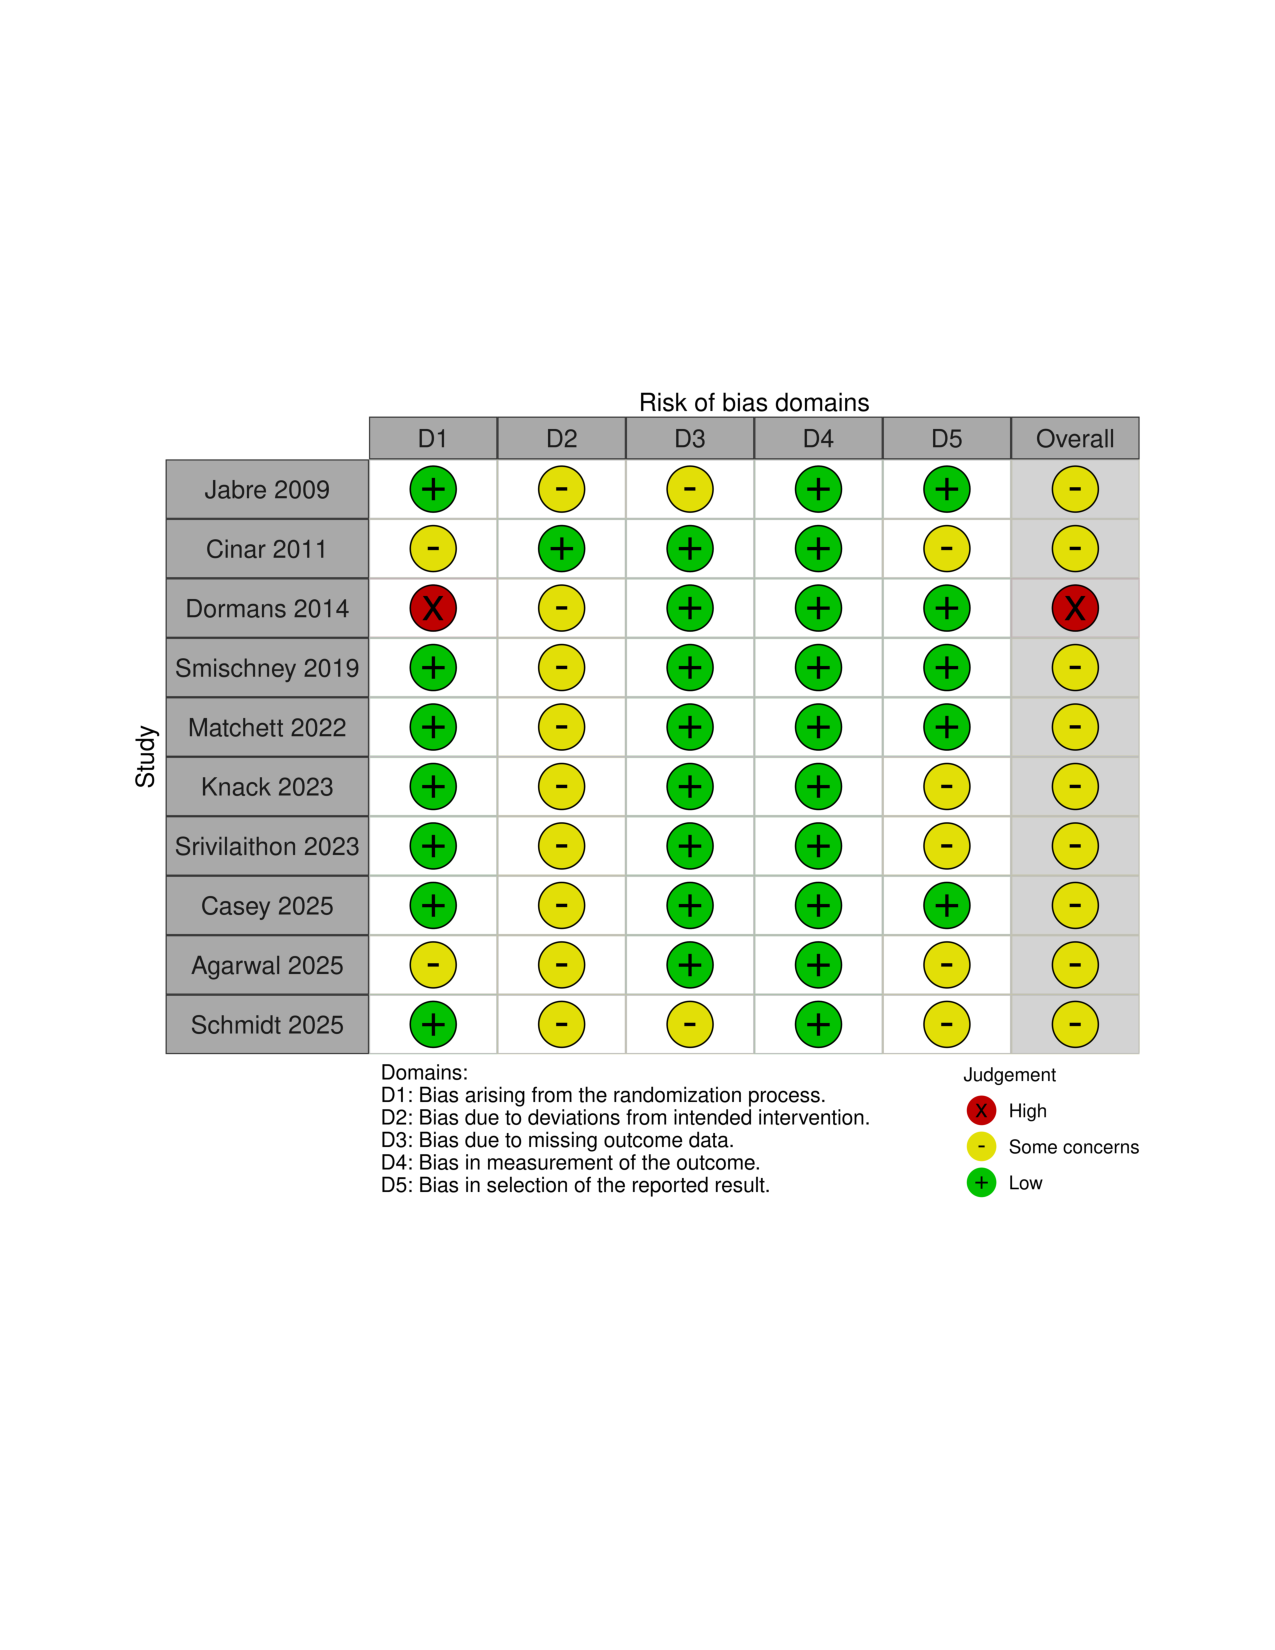
\includegraphics[width=\linewidth]{ROB2.pdf}
\end{minipage}
\hfill
\begin{minipage}[c]{0.48\linewidth}
\centering
\textbf{(B)}\\[4pt]
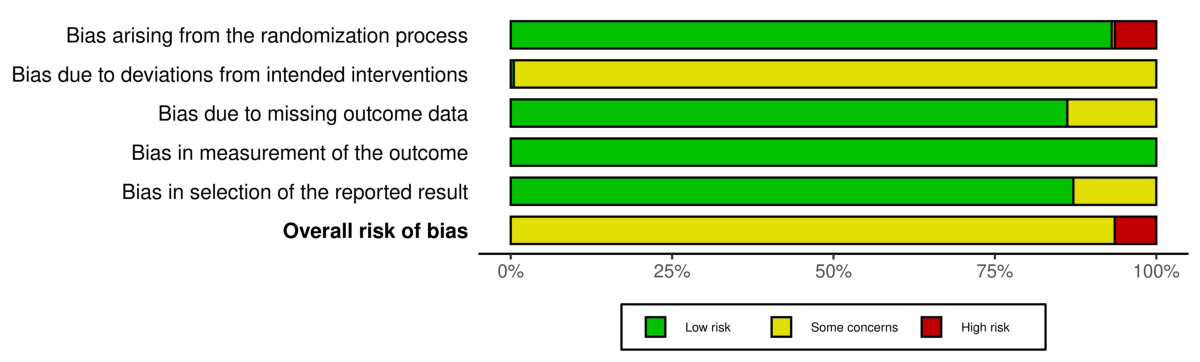
\includegraphics[width=\linewidth]{ROB2_2.pdf}
\end{minipage}
\vspace*{\fill}
\caption{\textbf{Risk of bias assessment (Cochrane RoB 2 tool).}
\textbf{(A)} Traffic-light plot showing domain-level judgements for each study. D1 = randomization process; D2 = deviations from intended interventions; D3 = missing outcome data; D4 = measurement of the outcome; D5 = selection of the reported result.
\textbf{(B)} Summary plot showing the distribution of risk-of-bias judgements across all studies. Nine studies were rated as ``some concerns'' and one (Dormans 2014) as ``high risk,'' driven by the cluster-randomized design and midazolam adjunct in the ketamine arm.}
\label{fig:rob}
\end{figure}
\end{landscape}

% --- FIGURE 3: Network + Forest ---
\begin{landscape}
\begin{figure}[p]
\singlespacing
\centering
\vspace*{\fill}

\includegraphics[height=0.78\textheight]{Figure3_network_forest.pdf}
\vspace*{\fill}
\caption{\textbf{Network geometry and pairwise meta-analysis of etomidate vs ketamine for short-term mortality.}
\textbf{(A)} Network geometry for the mortality analysis. Node size is proportional to the total number of patients randomized to each treatment. Edge thickness is proportional to the number of studies for each direct comparison. The etomidate--ketamine comparison dominates the network (8 of 10 studies).
\textbf{(B)} Forest plot showing the pairwise random-effects meta-analysis for etomidate vs ketamine (8 studies, 4,425 patients). Squares represent individual study estimates (size proportional to weight); the diamond represents the pooled estimate. The pooled OR was 1.01 (95\% CI 0.78--1.29; $I^2$ = 25\%), consistent with no difference in mortality between agents.}
\label{fig:main}
\end{figure}
\end{landscape}

\end{document}
